\section{Results and Discussion}
\subsection{Using solid-contact microelectrodes as potentiometric SECM probes}
Solid-contact electrodes have lower resistance, compared to their otherwise identical, liquid-contact counterparts.
This is due to two reasons.
The solid contact can be pushed down very close to the micropipette orifice, shortening the thickness of the highly resistive ion-selective membrane, and decreasing the overall electrode resistance.
The other reason is that instead of the internal solution -- which has high resistance --, a modified carbon fiber -- which has low resistance -- is used as the ion-to-electron transducer.
If $R$ is lower, $RC$ is lower, and the potentiometric cell becomes faster.

I constructed two Mg$^{2+}$-ion selective electrodes.
One used a liquid contact, and the other a solid contact.
Besides this difference, they were prepared identically.
Basic characterisation was performed for both.
Response characteristics were investigated by measuring the electrode resistance $R$, and the $\tau_{95}$ response time.
Calculated from the voltage divider measurements, electrode resistance was $4.8~$G$\ohm$ and $0.56~$G$\ohm$ for the liquid, and solid contact electrodes, respectively.
Based on these values, the solid contact electrode was expected to produce less distorted images with the same scanning parameters.

To confirm it, a Mg$^{2+}$ ion diffusion source model system was created, and the plane 100 $\upmu$m above the pipette orifice -- holding 0.1 M MgCl$_2$ solution -- was scanned with both electrodes.
Fig. \ref{fig:solid_liquid_pipette} shows the ISME images obtained using a liquid-contact (A), and a solid-contact (B), micropipette electrode.
Both 2D ISME maps were recorded at the same scan rate.
Visual inspection of the two images clearly shows significant image distortion in the X-direction with the liquid-contact ISME due its slower response as expected based on its higher resistance.
It can also be observed in the image scanned with the solid-contact electrode, although to a much less extent.
Another important feature to note in the images is the difference in the highest magnesium ion concentration observed with the two electrodes.
With the solid-contact microelectrode it's about $10^{-2.5}$ M.
On the other hand, with the conventional liquid-contact electrode, highest observed magnesium ion concentration is only about $10^{-3.4}$ M.
One possible reason for this is that the cell equipped with the liquid-contact electrode cannot keep up with the changes of the magnesium ion concentration at the micropipette orifice.

\begin{figure}
\centering
% trim = top left bottom right
\includegraphics[trim = 10mm 30mm 0mm 10mm, clip, width=0.35\textwidth, angle=-90]{img/mg_pipette/liquid_Mg.eps} \includegraphics[trim = 10mm 30mm 0mm 10mm, clip, width=0.35\textwidth, angle=-90]{img/mg_pipette/solid_Mg.eps}
\caption[SECM images displaying the Mg$^{2+}$ ion concentrations 100 $\upmu$m above the tip of a centered pipette source.]{SECM images displaying the Mg$^{2+}$ ion concentrations 100 $\upmu$m above the tip of a centered pipette source.
(A) liquid-contact, and (B) solid-contact.
Scan rate: 12.5 $\upmu$m/s.}
\label{fig:solid_liquid_pipette}
\end{figure}

One application that is included in my dissertation is the investigation of the galvanic corrosion of magnesium and its alloys. A solid contact magnesium ISME was used to map magnesium ion distribution above a corroding AZ63 magnesium-aluminium alloy.
Vertical Mg$^{2+}$ ion concentration distribution was determined at different instants in time of the corrosion process, with, and without coupling the Mg/Al and Fe samples.
Using the Mg$^{2+}$ concentration profiles, Mg$^{2+}$ flow rate from the Mg piece was possible to estimate:

\begin{equation}
\label{eq:corrosion_current}
        \Omega = 4 D C_s a
\end{equation}

where $\Omega$ is the amount of Mg$^{2+}$ released from the disc shaped Mg/Al surface, $D$ is the diffusion coefficient of Mg$^{2+}$, $C_s$ is the surface concentration of Mg$^{2+}$ (at the height $z$ = 0 $\upmu$m), $a$ is the radius of the Mg/Al sample.
As the only unknown variable in the equation above, $\Omega$ could be calculated.

Corrosion current between the Mg/Al sample and the Fe sample was also measured directly.
Using Faraday's law of electrolysis, corrosion current could be calculated from the first method.
It was in fairly good agreement with the SECM measurement.

\subsection{Optimization of scanning algorithms}
In the second and third approaches I exploit the properties of the potentiometric response function:

\begin{equation}
\label{eq:rc}
        E_{cell}(t_{e}) = E_{cell}(\infty) + [E_{cell}(0) - E_{cell}(\infty)]e^{-t_{e}/RC}
\end{equation}
where $E_{cell}(t)$ is the cell potential difference at time $t_{e}$, $E_{cell}(\infty)$ is the equilibrium cell potential difference, $E_{cell}(0)$ is the cell potential difference prior to the change.
The more different $E_{cell}(0)$ and $E_{cell}(\infty)$ are, the more the difference between $E_{cell}(\infty)$ and $E_{cell}(t_{e})$ will be.
Distortion of an image can be measured as an average of the differences between $E_{cell}(\infty)$ and $E_{cell}(t_{e})$ at each point.
It can be lowered by carefully optimizing scanning patterns and algorithms, so that the probe passes through borders between regions of high and low concentrations as few times as possible.

The results (Figure \ref{fig:simulations}) confirmed the presumption, that using the two new algorithms, images have less distortion, with higher similarity to the expected image.
I have confirmed the results with simulations as well.
Those results can be found in my dissertation.

\begin{figure}
\centering
% trim = top left bottom right
\includegraphics[trim = 10mm 30mm 0mm 10mm, clip, width=0.35\textwidth, angle=-90]{img/polar/meander.eps} \includegraphics[trim = 10mm 30mm 0mm 10mm, clip, width=0.35\textwidth, angle=-90]{img/polar/arc.eps}
\caption{Experimental SECM scans 100 $\upmu$m above the disc source with the (A) meander and the (B) arc scanning algorithms.
Measuring electrode was a pH-sensitive antimony micro-electrode.}
\label{fig:simulations}
\end{figure}

\subsection{Signal processing in potentiometric SECM}
In the third approach, I use the inverse of the potentiometric response function (Eq. \ref{eq:rc}) as deconvolution function.
Since the relationship between $t_e$, $E_{cell}(0)$, $E_{cell}(t_e)$ and $E_{cell}(\infty)$ is known, a prediction for the only unknown $E_{cell}(\infty)$ can be calculated.


\begin{figure}
\centering
% trim = top left bottom right
\includegraphics[trim = 10mm 30mm 0mm 10mm, clip, width=0.35\textwidth, angle=-90]{img/pH_2D_Sb/13121313.eps}\includegraphics[trim = 10mm 30mm 0mm 10mm, clip, width=0.35\textwidth, angle=-90]{img/pH_2D_Sb/13121313_deconvoluted.eps}%\includegraphics[trim = 20mm 30mm 0mm 20mm, clip, width=0.3\textwidth, angle=-90]{13121313_diff.eps}
\caption{SECM pH image before (A) and after (B) deconvolution.
Scan conducted with the antimony microelectrode.
Note the different potential scales.
Deconvolution restores not only the shape of the concentration profile, but the magnitude of the peak as well.
The raster scan pattern was used with the meander algorithm starting in the bottom left corner of the image.}
\label{fig:deconvolution}
\end{figure}

2D SECM scan was performed above a circular graphite anode (Fig. \ref{fig:deconvolution}A), with the meander scanning algorithm.
Line blur distortion in the raw images is visible along the alternating scanlines used by the meander scanning algorithm.
By deconvoluting the image, the expected potential map can be obtained (Fig. \ref{fig:deconvolution}B). 

Not only the circular shape of the target in the images is restored, but the peak value above the center of the target as well.
Maximum value in the raw scans was around $-300$ mV, whereas in the deconvoluted image, it was about $-260$ mV, with a significant difference between the two.
I have confirmed the validity of the deconvoluted values by very slow line scans. 

I obtained similar results with ionophore based ion selective micropipettes, which can be found in my dissertation. I haven't included those results here, due to the compact format of this booklet.

As an example of the application of the technique, corroding carbon steel was imaged.
As expected, the image was distorted, and without any processing evaluation proved to be difficult.
The irregular shape of the target was recognisable after, but not before the deconvolution.
The difference between the original and the processed image was quite large.
Without any processing, pH would have been misestimated by about 1 pH unit.
A different conclusion can be drawn based on the raw, and the deconvoluted image.

Another studied technique was blind deconvolution. This is the technique of deconvoluting measured data without the complete knowledge of the transfer function that describes the convolution.
To explore this possibility, I deconvoluted a pH image using the deconvolution function with several different time-constant substituations, including the measured one.

The best result could be easily recognized just by visual inspection, and it was the one that was deconvoluted by the correct, measured time-constant.
A more advanced method would be a statistical approach, where one would try to detect any correlation between the scanning algorithm -- taking into account the scan direction -- and the image, and choose the deconvoluted image with the least correlation.

\subsection{The effect of electric field on potentiometric SECM images}

During galvanic corrosion, ions are being released from the anode.
The measured potential of an ion selective microelectrode is thought to depend only on the activity of the primary ion.
However, an electric field is also formed as a result of the potential difference between the surfaces of the galvanic pair, which has a direct influence on the potential of the measuring microelectrode. The measured potential is the sum of these two contributions:

\begin{equation}
\Delta E=E_M-E_R + (\phi_M - \phi_R)
\label{eq:potential}
\end{equation}

where $\Delta E$ is the measured potential difference, $E_M$ and $E_R$ is the potential of the measuring and the reference electrode, and $\phi_M$ and $\phi_R$ are the local potentials in the electric field at the measuring and reference electrodes, respectively.

There are multiple papers featuring contradictory results obtained by studying system where a strong electric field is present. These contradictory results can be explained by a contribution of the electric field that is formed during these experiments. 

\begin{figure}
\centering
\begin{tikzpicture}
\begin{axis}[ymin=-75, ymax=200, xmin=0, xmax=680, xlabel={time, s}, ylabel={E, mV vs Ag/AgCl/ 3M KCl}, clip marker paths=true, width=7cm, height=7cm, legend style={draw=none}, legend cell align=left]
\addplot [domain=-30:100, color=red, mark=*] table {data/field/on_off_100.txt};
\addplot [domain=-30:100, color=blue, mark=*] table {data/field/on_off_1000.txt};
%\node[anchor=north east] at (rel axis cs:0.98,0.98) {B};
\node[red, above right] at (axis cs:10,20) {h = 100 $\upmu$m};
\node[blue, above right] at (axis cs:10,-50) {h = 1000 $\upmu$m};
\draw [black, ->] (axis cs:320,125) -- (axis cs:320,100);
\node[black, above] at (axis cs:320,125) {on};
\draw [black, ->] (axis cs:460,125) -- (axis cs:460,100);
\node[black, above] at (axis cs:460,125) {off};
\end{axis}
\end{tikzpicture}
\caption{Stationary recordings above the center of the AZ63 target with the ISME placed at: red = 100 $\upmu$m, blue = 1000 $\upmu$m distance from the metal. On/off denote the moment when galvanic coupling was either established or ceased. Temporal resolution was 1 Hz.}
\label{fig:approach}
\end{figure}

The ISME was maintained at a constant height from the metal surface, and its potential was recorded as a function of time, while the galvanic connection was established between the two metals (Fig. \ref{fig:approach}).
Thus, the tip was first positioned 100 $\upmu$m above the center of the AZ63 wire (red curve in Fig. \ref{fig:approach}), and for about 300 s the spontaneous corrosion of the alloy sample was recorded.
Then, the galvanic connection was established, and a sharp increase in potential of about 70 mV could be observed.
This change would correspond to a two orders of magnitude increase of Mg$^{2+}$ activity in a very short period of time.
When the galvanic connection was removed, a potential change of the same magnitude, though opposite direction could be observed.
In order to discard the possibility that this rise could be still explained by an abrupt release of Mg$^{2+}$ from the surface, the experiment was repeated while the tip was positioned 1000 $\upmu$m above the target (blue curve in Fig. \ref{fig:approach}).
A very similar sequence of potential changes could be observed, despite the big separation between the probe and the corroding sample.
The only plausible explanation is that the abrupt change in the recorded potential is due to the electric field developed between the two metals. 

The effect of the electric field in certain potentiometric SECM experiments has been demonstrated experimentally, as suspected by certain researchers in corrosion science for some time.
A strong electric field is formed around galvanic coupling of dissimilar metals, that causes significant over- or underestimations of the real primary ion activity.
The reason for this feature is that the electric field has a direct influence on the measured potential at the ISME.
